\chapter{Desarrollo del código}
\label{chap:desarrollo-codigo}
En la figura \ref{fig:org2aac9fc}, se muestra el proceso de cálculo que sigue el paquete a la hora de obtener la estimación de la producción del sistema fotovoltaico.
\begin{figure}[]
\centering
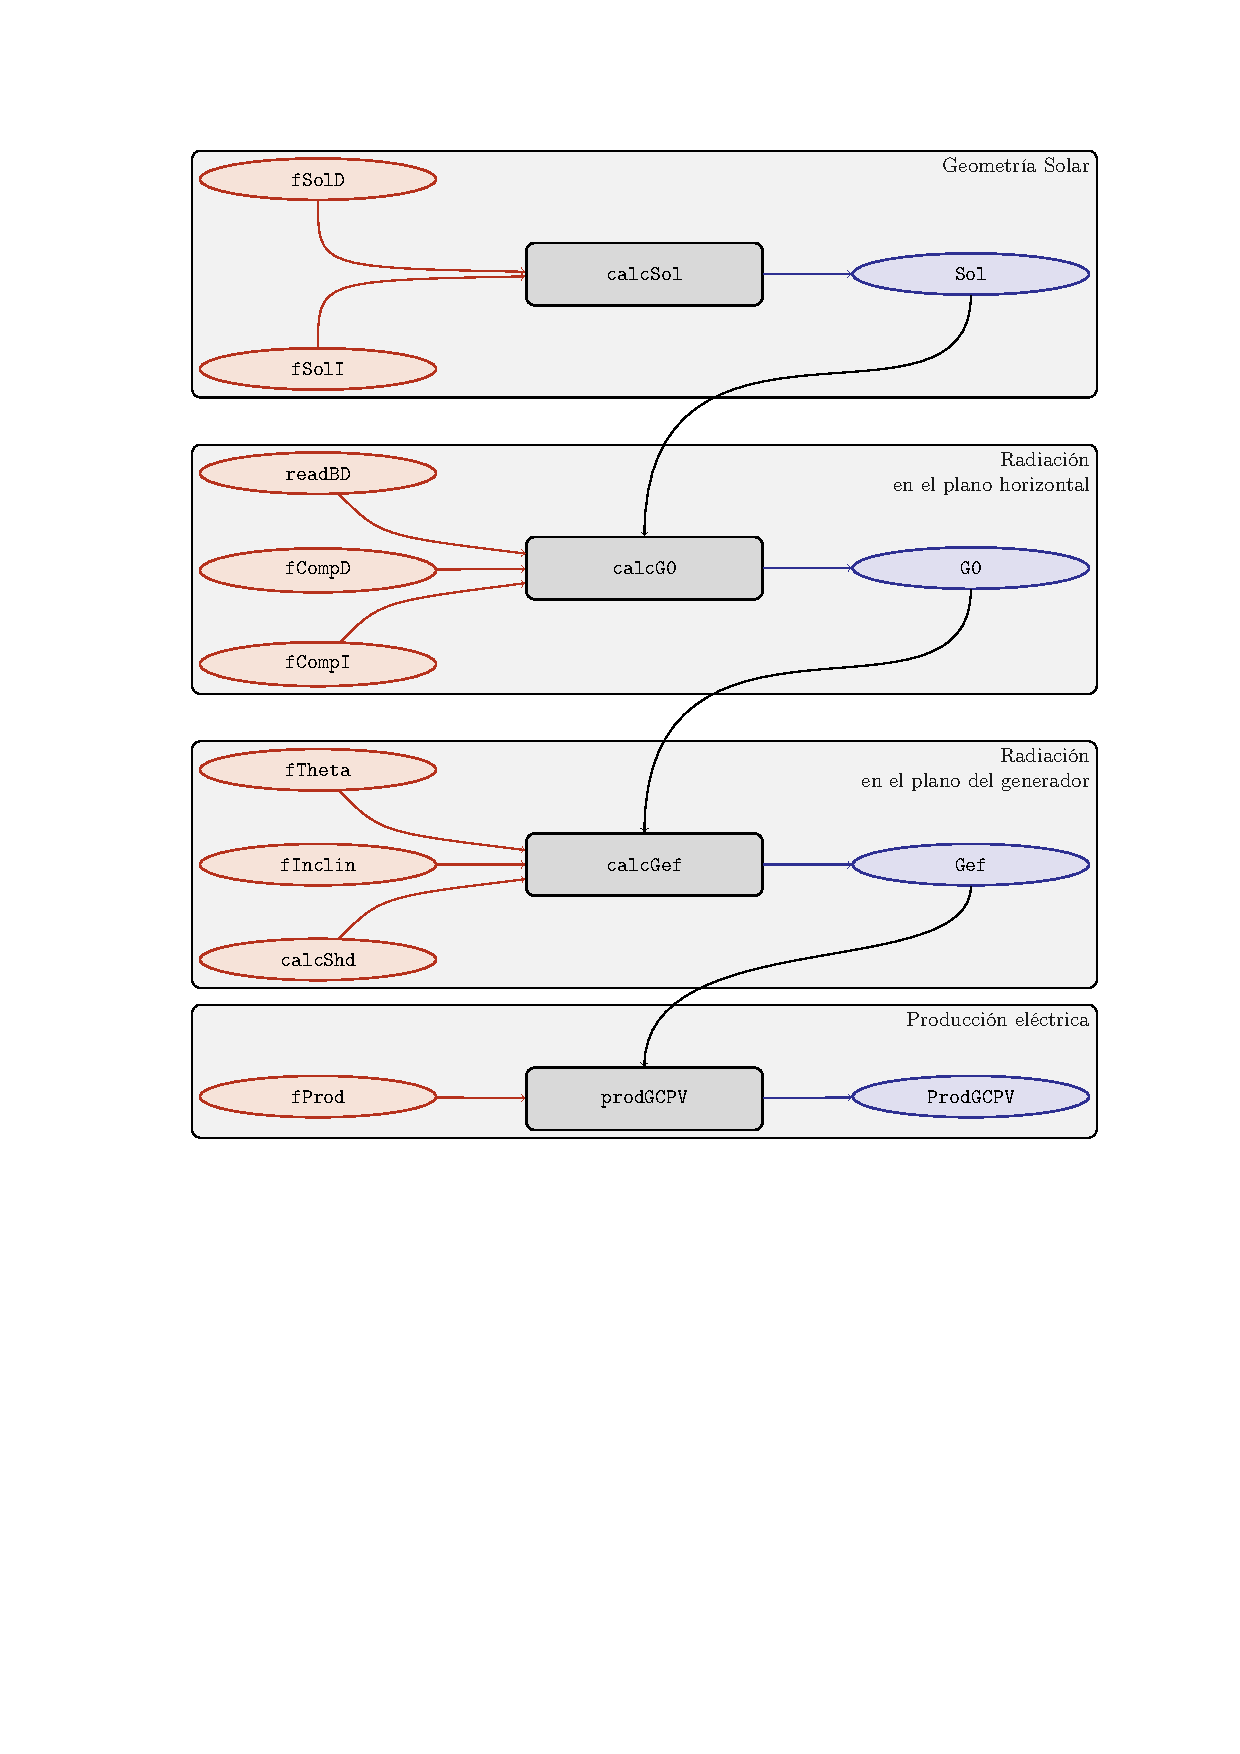
\includegraphics[keepaspectratio,width=0.8\textwidth,height=0.5\textheight]{figuras/procedure.pdf}
\caption{\label{fig:org2aac9fc}Proceso de cálculo de las funciones de \texttt{solaR2}}
\end{figure}
A la hora de estimar la producción, el programa sigue los siguientes procesos:
\section{Geometría solar}
\label{sec:org8696c04}
\label{sec:geometria-solar}
Para calcular la geometría que definen las posiciones de la Tierra y el Sol, \texttt{solaR2} se vale de una función constructora, \texttt{calcSol} [\ref{subsec:calcsol}], la cual mediante las funciones \texttt{fSolD} [\ref{subsec:fsold}] y \texttt{fSolI} [\ref{subsec:fsoli}] cálcula todos los ángulos y componentes que caracterizan la geometría solar.
\begin{figure}[]
\centering
\includegraphics[keepaspectratio,width=\textwidth,height=0.5\textheight]{figuras/calcSol.pdf}
\caption{Cálculo de la geometría solar mediante la función \texttt{calcSol}, la cual unifica las funciones \texttt{fSolD} y \texttt{fSolI} resultando en un objeto clase \texttt{Sol} el cual contiene toda la información geométrica necesaria para realizar las siguientes estimaciones. \label{fig:calcSol}}
\end{figure}

Como se puede ver en la figura \ref{fig:calcSol}, \texttt{calcSol} funcia gracias a las siguientes funciones:
\begin{itemize}
\item \texttt{fSolD}: la cual, a partir de la latitud (\(\phi\)), computa la geometría a nivel diario, es decir, los ángulos y componentes que se pueden calcular en cada día independiente.

estas son:
\begin{itemize}
\item Declinación (\(\delta\)): calculada a partir de la función \texttt{declination}\footnote{Todas las funciones mencionadas en este punto, se encuentran en el apartado \ref{subsec:utils-angles}.}.
\item Excentricidad (\(\epsilon_o\)): obtenida mediante la función \texttt{eccentricity}.
\item Ecuación del tiempo (\(EoT\)): obtenida mediante la función \texttt{eot}.
\item Ángulo del amanecer (\(\omega_s\)): calculada a partir de la función \texttt{sunrise}.
\item Irradiancia diaria extra-atmosférica (\(B_{0d}(0)\)): obtenida a paritr de la función \texttt{bo0d}.
\end{itemize}
\end{itemize}
\begin{lstlisting}[numbers=left,language=r,label= ,caption= ,captionpos=b]
lat <- 40
BTd <- fBTd(mode = 'prom')
fSolD(lat = lat, BTd = BTd)
show(solD)
\end{lstlisting}

\begin{verbatim}
Key: <Dates>
         Dates   lat        decl        eo           EoT        ws      Bo0d
        <IDat> <num>       <num>     <num>         <num>     <num>     <num>
 1: 2024-01-17  37.2 -0.36271754 1.0340422 -0.0455346238 -1.278593  4738.993
 2: 2024-02-14  37.2 -0.22850166 1.0259717 -0.0614793356 -1.393341  6137.388
 3: 2024-03-15  37.2 -0.03191616 1.0107943 -0.0368674274 -1.546560  8086.323
 4: 2024-04-15  37.2  0.17531794 0.9926547  0.0017482721 -1.705659  9921.357
 5: 2024-05-15  37.2  0.33246485 0.9775162  0.0143055938 -1.835976 11115.619
 6: 2024-06-10  37.2  0.40257826 0.9691480 -0.0007378952 -1.899934 11573.907
 7: 2024-07-18  37.2  0.36439367 0.9675489 -0.0263454380 -1.864521 11257.133
 8: 2024-08-18  37.2  0.22407398 0.9758022 -0.0111761118 -1.744657 10183.208
 9: 2024-09-18  37.2  0.02730595 0.9907919  0.0342189964 -1.591529  8508.642
10: 2024-10-19  37.2 -0.17900474 1.0088406  0.0689613044 -1.433019  6554.218
11: 2024-11-18  37.2 -0.33862399 1.0245012  0.0575423573 -1.300179  4951.750
12: 2024-12-13  37.2 -0.40478283 1.0328516  0.0158622941 -1.239567  4284.472
\end{verbatim}

Además, \texttt{fSolD} permite seleccionar el método de cáculo entre los propuestos por 4 autores diferentes (\texttt{cooper} \cite{Cooper1969}, \texttt{spencer} \cite{Spencer1971}, \texttt{strous} \cite{Strous2011}, \texttt{michalsky} \cite{Michalsky1988})(el valor por defecto es \texttt{michalsky}):
\begin{lstlisting}[numbers=left,language=r,label= ,caption= ,captionpos=b]
solD_cooper <- fSolD(lat = lat, BTd = BTd, method = 'cooper')
show(solD_cooper)
\end{lstlisting}

\begin{verbatim}
Key: <Dates>
         Dates   lat        decl        eo           EoT        ws      Bo0d
        <IDat> <num>       <num>     <num>         <num>     <num>     <num>
 1: 2024-01-17    40 -0.36506987 1.0315970 -0.0455346238 -1.244322  4225.330
 2: 2024-02-14    40 -0.23770977 1.0235842 -0.0614793356 -1.366063  5581.840
 3: 2024-03-15    40 -0.04219743 1.0091112 -0.0368674274 -1.535360  7621.789
 4: 2024-04-15    40  0.17074888 0.9917107  0.0017482721 -1.715990  9677.015
 5: 2024-05-15    40  0.33214647 0.9770196  0.0143055938 -1.864424 11059.743
 6: 2024-06-10    40  0.40292516 0.9690335 -0.0007378952 -1.936560 11599.039
 7: 2024-07-18    40  0.36346384 0.9684861 -0.0263454380 -1.895642 11244.195
 8: 2024-08-18    40  0.21721704 0.9778484 -0.0111761118 -1.757060  9992.309
 9: 2024-09-18    40  0.01056696 0.9933706  0.0342189964 -1.579664  8057.402
10: 2024-10-19    40 -0.19902155 1.0107363  0.0689613044 -1.400739  5932.854
11: 2024-11-18    40 -0.34965673 1.0247443  0.0575423573 -1.259840  4363.600
12: 2024-12-13    40 -0.40651987 1.0315970  0.0158622941 -1.201207  3779.136
\end{verbatim}

\begin{lstlisting}[numbers=left,language=r,label= ,caption= ,captionpos=b]
solD_spencer <- fSolD(lat = lat, BTd = BTd, method = 'spencer')
show(solD_spencer)
\end{lstlisting}

\begin{verbatim}
Key: <Dates>
         Dates   lat        decl        eo           EoT        ws      Bo0d
        <IDat> <num>       <num>     <num>         <num>     <num>     <num>
 1: 2024-01-17    40 -0.36483670 1.0340422 -0.0455346238 -1.244559  4237.879
 2: 2024-02-14    40 -0.23199205 1.0259717 -0.0614793356 -1.371241  5657.973
 3: 2024-03-15    40 -0.03563921 1.0107943 -0.0368674274 -1.540874  7704.956
 4: 2024-04-15    40  0.17171286 0.9926547  0.0017482721 -1.716832  9695.800
 5: 2024-05-15    40  0.33007088 0.9775162  0.0143055938 -1.862390 11046.417
 6: 2024-06-10    40  0.40208757 0.9691480 -0.0007378952 -1.935671 11593.079
 7: 2024-07-18    40  0.36657157 0.9675489 -0.0263454380 -1.898797 11260.952
 8: 2024-08-18    40  0.22748717 0.9758022 -0.0111761118 -1.766286 10069.634
 9: 2024-09-18    40  0.03143967 0.9907919  0.0342189964 -1.597189  8253.467
10: 2024-10-19    40 -0.17549393 1.0088406  0.0689613044 -1.421454  6177.523
11: 2024-11-18    40 -0.33679169 1.0245012  0.0575423573 -1.272602  4501.910
12: 2024-12-13    40 -0.40419949 1.0328516  0.0158622941 -1.203679  3808.563
\end{verbatim}

\begin{lstlisting}[numbers=left,language=r,label= ,caption= ,captionpos=b]
solD_strous <- fSolD(lat = lat, BTd = BTd, method = 'cooper')
show(solD_strous)
\end{lstlisting}

\begin{verbatim}
Key: <Dates>
         Dates   lat        decl        eo           EoT        ws      Bo0d
        <IDat> <num>       <num>     <num>         <num>     <num>     <num>
 1: 2024-01-17    40 -0.36506987 1.0315970 -0.0455346238 -1.244322  4225.330
 2: 2024-02-14    40 -0.23770977 1.0235842 -0.0614793356 -1.366063  5581.840
 3: 2024-03-15    40 -0.04219743 1.0091112 -0.0368674274 -1.535360  7621.789
 4: 2024-04-15    40  0.17074888 0.9917107  0.0017482721 -1.715990  9677.015
 5: 2024-05-15    40  0.33214647 0.9770196  0.0143055938 -1.864424 11059.743
 6: 2024-06-10    40  0.40292516 0.9690335 -0.0007378952 -1.936560 11599.039
 7: 2024-07-18    40  0.36346384 0.9684861 -0.0263454380 -1.895642 11244.195
 8: 2024-08-18    40  0.21721704 0.9778484 -0.0111761118 -1.757060  9992.309
 9: 2024-09-18    40  0.01056696 0.9933706  0.0342189964 -1.579664  8057.402
10: 2024-10-19    40 -0.19902155 1.0107363  0.0689613044 -1.400739  5932.854
11: 2024-11-18    40 -0.34965673 1.0247443  0.0575423573 -1.259840  4363.600
12: 2024-12-13    40 -0.40651987 1.0315970  0.0158622941 -1.201207  3779.136
\end{verbatim}

\begin{itemize}
\item \texttt{fSolI}: toma los resultados obtenidos en \texttt{fSolD} y calcula la geometría a nivel intradiario, es decir, aquella que se puede calcular en unidades de tiempo menores a los días.
estas son:
\begin{itemize}
\item La hora solar o tiempo solar verdadero (\(\omega\)): calculada a partir de la función \texttt{sunHour}.
\item Los momentos del día en los que es de noche (\(night\)): calculada a partir del resultado anterior y de el ángulo del amanecer (cálculada en \texttt{fSolD})\footnote{Cuando la hora solar verdadera excede los ángulos en los que amanece y anochece (\(|\omega|>=|\omega_s|\)), el Sol queda por debajo de la línea del horizonte, por lo que es de noche.}.
\item El coseno del ángulo cenital solar (\(cos(\theta_{zs})\)): obtenida a partir de la función \texttt{zenith}.
\item La altura solar (\(\gamma_s\)): obtenida a partir del resultado anterior\footnote{\(\gamma_s=asin(cos(\theta_s))\).}.
\item El ángulo zenital solar (\(\theta_{zs}\)): calculada mediante la función \texttt{azimuth}.
\item La irradiancia extra-atmosférica (\(B_0(0)\)): calculada mediante el coseno del ángulo cenital, la constante solar (\(B_0\)) y la excentridad (cálculada en \texttt{fSolD}) [ecuación \ref{eq:irrad_horiz}].
\end{itemize}
\end{itemize}
\begin{lstlisting}[numbers=left,language=r,label= ,caption= ,captionpos=b]
solI <- fSolI(solD = solD[1], sample = 'hour') #Computo solo un día a fin mejorar la visualización
show(solI)
\end{lstlisting}

\begin{verbatim}
Index: <night>
                  Dates   lat           w  night      cosThzS          AlS         AzS       Bo0
                 <POSc> <num>       <num> <lgcl>        <num>        <num>       <num>     <num>
 1: 2024-01-17 00:00:00  37.2  3.09905026   TRUE -0.958552332 -1.281876984  3.00157749   0.00000
 2: 2024-01-17 01:00:00  37.2 -2.92239722   TRUE -0.941407376 -1.226779122 -2.49462689   0.00000
 3: 2024-01-17 02:00:00  37.2 -2.66065932   TRUE -0.874749489 -1.064918604 -2.03862388   0.00000
 4: 2024-01-17 03:00:00  37.2 -2.39892132   TRUE -0.763119126 -0.868125900 -1.77932134   0.00000
 5: 2024-01-17 04:00:00  37.2 -2.13718324   TRUE -0.614120126 -0.661270606 -1.59701536   0.00000
 6: 2024-01-17 05:00:00  37.2 -1.87544507   TRUE -0.437901763 -0.453263434 -1.44469585   0.00000
 7: 2024-01-17 06:00:00  37.2 -1.61370681   TRUE -0.246467423 -0.249033534 -1.30093496   0.00000
 8: 2024-01-17 07:00:00  37.2 -1.35196846   TRUE -0.052856976 -0.052881619 -1.15283370   0.00000
 9: 2024-01-17 08:00:00  37.2 -1.09023003  FALSE  0.129741461  0.130108233 -0.99014548 183.39419
10: 2024-01-17 09:00:00  37.2 -0.82849151  FALSE  0.288889848  0.293067041 -0.80329847 408.35612
11: 2024-01-17 10:00:00  37.2 -0.56675290  FALSE  0.413747472  0.426566560 -0.58400587 584.84684
12: 2024-01-17 11:00:00  37.2 -0.30501420  FALSE  0.495809380  0.518766586 -0.32921922 700.84427
13: 2024-01-17 12:00:00  37.2 -0.04327541  FALSE  0.529485721  0.557994217 -0.04769723 748.44699
14: 2024-01-17 13:00:00  37.2  0.21846346  FALSE  0.512482515  0.538073327  0.23821864 724.41235
15: 2024-01-17 14:00:00  37.2  0.48020243  FALSE  0.445957919  0.462244212  0.50355560 630.37745
16: 2024-01-17 15:00:00  37.2  0.74194148  FALSE  0.334443348  0.341014503  0.73469016 472.74762
17: 2024-01-17 16:00:00  37.2  1.00368062  FALSE  0.185534810  0.186616094  0.93148844 262.26008
18: 2024-01-17 17:00:00  37.2  1.26541985  FALSE  0.009375501  0.009375638  1.10112996  13.25261
19: 2024-01-17 18:00:00  37.2  1.52715917   TRUE -0.182035120 -0.183055757  1.25297092   0.00000
20: 2024-01-17 19:00:00  37.2  1.78889857   TRUE -0.375658695 -0.385107424  1.39694027   0.00000
21: 2024-01-17 20:00:00  37.2  2.05063807   TRUE -0.558306105 -0.592342658  1.54466726   0.00000
22: 2024-01-17 21:00:00  37.2  2.31237766   TRUE -0.717535874 -0.800258081  1.71368519   0.00000
23: 2024-01-17 22:00:00  37.2  2.57411733   TRUE -0.842501657 -1.001910427  1.93928567   0.00000
24: 2024-01-17 23:00:00  37.2  2.83585709   TRUE -0.924691065 -1.180223341  2.30977400   0.00000
                  Dates   lat           w  night      cosThzS          AlS         AzS       Bo0
\end{verbatim}

Además, como los datos nocturnos aportan poco a los cálculos que atañen a este proyecto, \texttt{fSolI} presenta la posibilidad de eliminar estos datos con el argumento \texttt{keep.night}.
\begin{lstlisting}[numbers=left,language=r,label= ,caption= ,captionpos=b]
solI_nigth <- fSolI(solD = solD[1], sample = 'hour', keep.night = FALSE)
show(solI_nigth)
\end{lstlisting}

\begin{verbatim}
                  Dates   lat           w  night     cosThzS         AlS         AzS       Bo0
                 <POSc> <num>       <num> <lgcl>       <num>       <num>       <num>     <num>
 1: 2024-01-17 08:00:00  37.2 -1.09023003  FALSE 0.129741461 0.130108233 -0.99014548 183.39419
 2: 2024-01-17 09:00:00  37.2 -0.82849151  FALSE 0.288889848 0.293067041 -0.80329847 408.35612
 3: 2024-01-17 10:00:00  37.2 -0.56675290  FALSE 0.413747472 0.426566560 -0.58400587 584.84684
 4: 2024-01-17 11:00:00  37.2 -0.30501420  FALSE 0.495809380 0.518766586 -0.32921922 700.84427
 5: 2024-01-17 12:00:00  37.2 -0.04327541  FALSE 0.529485721 0.557994217 -0.04769723 748.44699
 6: 2024-01-17 13:00:00  37.2  0.21846346  FALSE 0.512482515 0.538073327  0.23821864 724.41235
 7: 2024-01-17 14:00:00  37.2  0.48020243  FALSE 0.445957919 0.462244212  0.50355560 630.37745
 8: 2024-01-17 15:00:00  37.2  0.74194148  FALSE 0.334443348 0.341014503  0.73469016 472.74762
 9: 2024-01-17 16:00:00  37.2  1.00368062  FALSE 0.185534810 0.186616094  0.93148844 262.26008
10: 2024-01-17 17:00:00  37.2  1.26541985  FALSE 0.009375501 0.009375638  1.10112996  13.25261
\end{verbatim}

Finalmente, estas dos funciones, como se muestra en la figura \ref{fig:calcSol}, convergen en la función \texttt{calcSol}, dando como resultado un objeto de clase \texttt{Sol}. Este objeto muestra un sumario de ambos elementos junto con la latitud de los cálculos.
\begin{lstlisting}[numbers=left,language=r,label= ,caption= ,captionpos=b]
sol <- calcSol(lat = lat, BTd = BTd, sample = 'hour')
print(sol)
\end{lstlisting}

\begin{verbatim}
Object of class Sol 

Latitude:  40 degrees

Daily values:
     Dates                 decl                 eo              EoT                   ws        
 Min.   :2024-01-17   Min.   :-0.404783   Min.   :0.9675   Min.   :-0.0614793   Min.   :-1.936  
 1st Qu.:2024-04-07   1st Qu.:-0.256032   1st Qu.:0.9771   1st Qu.:-0.0289759   1st Qu.:-1.789  
 Median :2024-06-29   Median :-0.002305   Median :1.0007   Median : 0.0005052   Median :-1.569  
 Mean   :2024-07-01   Mean   :-0.001618   Mean   :1.0009   Mean   : 0.0008748   Mean   :-1.569  
 3rd Qu.:2024-09-25   3rd Qu.: 0.251172   3rd Qu.:1.0249   3rd Qu.: 0.0204515   3rd Qu.:-1.348  
 Max.   :2024-12-13   Max.   : 0.402578   Max.   :1.0340   Max.   : 0.0689613   Max.   :-1.203  
      Bo0d      
 Min.   : 3802  
 1st Qu.: 5393  
 Median : 7978  
 Mean   : 7834  
 3rd Qu.:10295  
 Max.   :11597  

Intradaily values: 
     Dates                           w                night            cosThzS         
 Min.   :2024-01-17 00:00:00   Min.   :-3.1393050   Mode :logical   Min.   :-0.957052  
 1st Qu.:2024-04-07 11:45:00   1st Qu.:-1.5692285   FALSE:145       1st Qu.:-0.469842  
 Median :2024-06-29 11:30:00   Median : 0.0010871   TRUE :143       Median : 0.005586  
 Mean   :2024-07-01 15:30:00   Mean   : 0.0009975                   Mean   :-0.001012  
 3rd Qu.:2024-09-26 11:15:00   3rd Qu.: 1.5716412                   3rd Qu.: 0.472405  
 Max.   :2024-12-13 23:00:00   Max.   : 3.1413972                   Max.   : 0.956640  
      AlS                 AzS                 Bo0          
 Min.   :-1.276658   Min.   :-3.139232   Min.   :   0.000  
 1st Qu.:-0.489119   1st Qu.:-1.572101   1st Qu.:   0.000  
 Median : 0.005586   Median : 0.003240   Median :   7.746  
 Mean   :-0.001250   Mean   : 0.001007   Mean   : 326.418  
 3rd Qu.: 0.492019   3rd Qu.: 1.571070   3rd Qu.: 663.617  
 Max.   : 1.275239   Max.   : 3.141341   Max.   :1267.381
\end{verbatim}

\section{Datos meteorológicos}
\label{sec:org6aa4dc1}
\label{sec:datos-meteorologicos}
Para el procesamiento de datos meteorologicos, \texttt{solaR2} provee una serie de funciones\footnote{Las funciones comentadas en este apartado, se recogen en la sección \ref{subsec:meteoreaders}} que son capaces de leer todo tipo de datos. Estos datos se procesan y se almacenan en un objeto de tipo \texttt{Meteo} tal y como se ve en la figura \ref{fig:meteo}. Estas funciones son:
\begin{figure}[]
\centering
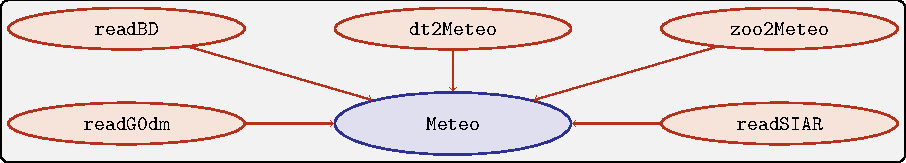
\includegraphics[keepaspectratio,width=\textwidth,height=0.5\textheight]{figuras/meteo.pdf}
\caption{Los datos meteorologicas se pueden leer mediante las funciones \texttt{readG0dm}, \texttt{readBD}, \texttt{dt2Meteo}, \texttt{zoo2Meteo} y \texttt{readSIAR} las cuales procesan estos datos y los almacenan en un objeto de clase \texttt{Meteo}. \label{fig:meteo}}
\end{figure}
\begin{itemize}
\item \texttt{readG0dm}: Esta función construye un objeto \texttt{Meteo} a partir de 12 valores de medias mensuales de irradiación.
\end{itemize}
\begin{lstlisting}[numbers=left,language=r,label= ,caption= ,captionpos=b]
G0dm = c(2.766,3.491,4.494,5.912,6.989,7.742,
         7.919,7.027,5.369,3.562,2.814,2.179) * 1000;
Ta = c(10, 14.1, 15.6, 17.2, 19.3, 21.2,
       28.4, 29.9, 24.3, 18.2, 17.2, 15.2)
BD <- readG0dm(G0dm = G0dm, Ta = Ta, lat = 37.2)
print(BD)
\end{lstlisting}

\begin{verbatim}
Object of class  Meteo 

Source of meteorological information: prom- 
Latitude of source:  37.2 degrees

Meteorological Data:
     Dates                 G0d             Ta       
 Min.   :2024-01-17   Min.   :2179   Min.   :10.00  
 1st Qu.:2024-04-07   1st Qu.:3322   1st Qu.:15.50  
 Median :2024-06-29   Median :4932   Median :17.70  
 Mean   :2024-07-01   Mean   :5022   Mean   :19.22  
 3rd Qu.:2024-09-25   3rd Qu.:6998   3rd Qu.:21.98  
 Max.   :2024-12-13   Max.   :7919   Max.   :29.90
\end{verbatim}

\begin{itemize}
\item \texttt{readBD}: Esta familia de funciones puede leer ficheros de datos y transformarlos en un objeto de clase \texttt{Meteo}. Se dividen en:
\begin{itemize}
\item \texttt{readBDd}: Procesa datos meteorológicos de tipo diarios.
\end{itemize}
\begin{lstlisting}[numbers=left,language=r,label= ,caption= ,captionpos=b]
## Se utiliza un archivo alojado en el
## github del tutor de este proyecto 
myURL <-"https://raw.githubusercontent.com/oscarperpinan/R/master/data/aranjuez.csv"
download.file(myURL, 'data/aranjuez.csv', quiet = TRUE)
BDd <- readBDd(file = 'data/aranjuez.csv', lat = lat,
               format = '%Y-%m-%d', header = TRUE,
               fill = TRUE, dec = '.', sep = ',', dates.col = '',
               ta.col = 'TempAvg', g0.col = 'Radiation', keep.cols = TRUE)
print(BDd)
\end{lstlisting}

\begin{verbatim}
Object of class  Meteo 

Source of meteorological information: bd-data/aranjuez.csv 
Latitude of source:  40 degrees

Meteorological Data:
     Dates                  G0               Ta            TempMin           TempMax      
 Min.   :2004-01-01   Min.   : 0.277   Min.   :-5.309   Min.   :-12.980   Min.   :-2.362  
 1st Qu.:2005-12-29   1st Qu.: 9.370   1st Qu.: 7.692   1st Qu.:  1.515   1st Qu.:14.530  
 Median :2008-01-09   Median :16.660   Median :13.810   Median :  7.170   Median :21.670  
 Mean   :2008-01-03   Mean   :16.742   Mean   :14.405   Mean   :  6.888   Mean   :22.531  
 3rd Qu.:2010-01-02   3rd Qu.:24.650   3rd Qu.:21.615   3rd Qu.: 12.590   3rd Qu.:30.875  
 Max.   :2011-12-31   Max.   :32.740   Max.   :30.680   Max.   : 22.710   Max.   :41.910  
		      NA's   :13                        NA's   :4                         
    HumidAvg         HumidMax         WindAvg         WindMax            Rain              ET       
 Min.   : 19.89   Min.   : 35.88   Min.   :0.251   Min.   : 0.000   Min.   : 0.000   Min.   :0.000  
 1st Qu.: 47.04   1st Qu.: 81.60   1st Qu.:0.667   1st Qu.: 3.783   1st Qu.: 0.000   1st Qu.:1.168  
 Median : 62.58   Median : 90.90   Median :0.920   Median : 5.027   Median : 0.000   Median :2.758  
 Mean   : 62.16   Mean   : 87.22   Mean   :1.174   Mean   : 5.208   Mean   : 1.094   Mean   :3.091  
 3rd Qu.: 77.38   3rd Qu.: 94.90   3rd Qu.:1.431   3rd Qu.: 6.537   3rd Qu.: 0.200   3rd Qu.:4.926  
 Max.   :100.00   Max.   :100.00   Max.   :8.260   Max.   :10.000   Max.   :49.730   Max.   :8.564  
		  NA's   :13       NA's   :8       NA's   :128      NA's   :4        NA's   :18
\end{verbatim}

\begin{itemize}
\item \texttt{readBDi}: Procesa datos meteorológicos de tipo intradiarios.
\end{itemize}
\begin{lstlisting}[numbers=left,language=r,label= ,caption= ,captionpos=b]
myURL <- "https://raw.githubusercontent.com/oscarperpinan/R/master/data/NREL-Hawaii.csv"
download.file(myURL, 'data/NREL-Hawaii.csv', quiet = TRUE)
BDi <- readBDi(file = 'data/NREL-Hawaii.csv', lat = 19,
               format = "%d/%m/%Y %H:%M", header = TRUE,
               fill = TRUE, dec = '.', sep = ',',
               dates.col = 'DATE', times.col = 'HST',
               ta.col = 'Air Temperature [deg C]',
               g0.col = 'Global Horizontal [W/m^2]',
               keep.cols = TRUE)
print(BDi)
\end{lstlisting}

\begin{verbatim}
Object of class  Meteo 

Source of meteorological information: bdI-data/NREL-Hawaii.csv 
Latitude of source:  19 degrees

Meteorological Data:
     Dates                              G0                  Ta        Direct Normal [W/m^2]
 Min.   :2010-01-11 06:32:00.00   Min.   :   0.4769   Min.   :13.42   Min.   :  0.0        
 1st Qu.:2010-03-11 17:37:45.00   1st Qu.: 147.4328   1st Qu.:22.76   1st Qu.:  0.0        
 Median :2010-06-11 17:32:30.00   Median : 300.6510   Median :24.15   Median :270.3        
 Mean   :2010-06-26 11:55:22.63   Mean   : 370.5293   Mean   :23.64   Mean   :356.6        
 3rd Qu.:2010-09-11 17:34:15.00   3rd Qu.: 585.7402   3rd Qu.:25.24   3rd Qu.:715.2        
 Max.   :2010-12-11 17:46:00.00   Max.   :1172.3000   Max.   :28.12   Max.   :943.0        
 NA's   :4660                                                                              
 Diffuse Horizontal [W/m^2]
 Min.   :  0.4769          
 1st Qu.: 78.4636          
 Median :152.9320          
 Mean   :171.7706          
 3rd Qu.:246.3193          
 Max.   :586.3600
\end{verbatim}

\item \texttt{dt2Meteo}: Transforma un \texttt{data.table} o \texttt{data.frame} en un objeto de clase \texttt{Meteo}.
\end{itemize}
\begin{lstlisting}[numbers=left,language=r,label= ,caption= ,captionpos=b]
data(helios)
names(helios) <- c('Dates', 'G0d', 'TempMax', 'TempMin')
helios_meteo <- dt2Meteo(file = helios, lat = 40, type = 'bd')
print(helios_meteo)
\end{lstlisting}

\begin{verbatim}
Object of class  Meteo 

Source of meteorological information: bd-data.frame 
Latitude of source:  40 degrees

Meteorological Data:
     Dates                             G0d             TempMin           TempMax     
 Min.   :2009-01-01 00:00:00.00   Min.   :  325.6   Min.   :-37.500   Min.   : 1.41  
 1st Qu.:2009-04-08 12:00:00.00   1st Qu.: 2523.2   1st Qu.:  1.950   1st Qu.:14.41  
 Median :2009-07-07 00:00:00.00   Median : 4745.7   Median :  7.910   Median :23.16  
 Mean   :2009-07-04 21:29:54.93   Mean   : 4812.0   Mean   :  5.323   Mean   :22.59  
 3rd Qu.:2009-10-03 12:00:00.00   3rd Qu.: 7139.5   3rd Qu.: 15.105   3rd Qu.:31.06  
 Max.   :2009-12-31 00:00:00.00   Max.   :11253.9   Max.   : 24.800   Max.   :38.04  
       Ta         
 Min.   :-23.049  
 1st Qu.:  7.008  
 Median : 12.055  
 Mean   : 10.944  
 3rd Qu.: 19.472  
 Max.   : 28.619
\end{verbatim}

\begin{itemize}
\item \texttt{zoo2Meteo}: Transforma un objeto de clase \texttt{zoo}\footnote{Pese a que este proyecto trate de ``desligarse'' del paquete \texttt{zoo}, sigue siendo un paquete muy extendido. Por lo que es interesante tener una función así para que los usuarios tengan una mayor flexibilidad.} en un objeto de clase \texttt{Meteo}.
\end{itemize}
\begin{lstlisting}[numbers=left,language=r,label= ,caption= ,captionpos=b]
library(zoo)
bd_zoo <- read.csv.zoo('data/aranjuez.csv')
BD_zoo <- zoo2Meteo(file = bd_zoo, lat = 40)
print(BD_zoo)
\end{lstlisting}

\begin{verbatim}
Object of class  Meteo 

Source of meteorological information: bd-zoo-bd_zoo 
Latitude of source:  40 degrees

Meteorological Data:
    TempAvg          TempMax          TempMin           HumidAvg         HumidMax         WindAvg     
 Min.   :-5.309   Min.   :-2.362   Min.   :-12.980   Min.   : 19.89   Min.   : 35.88   Min.   :0.251  
 1st Qu.: 7.692   1st Qu.:14.530   1st Qu.:  1.515   1st Qu.: 47.04   1st Qu.: 81.60   1st Qu.:0.667  
 Median :13.810   Median :21.670   Median :  7.170   Median : 62.58   Median : 90.90   Median :0.920  
 Mean   :14.405   Mean   :22.531   Mean   :  6.888   Mean   : 62.16   Mean   : 87.22   Mean   :1.174  
 3rd Qu.:21.615   3rd Qu.:30.875   3rd Qu.: 12.590   3rd Qu.: 77.38   3rd Qu.: 94.90   3rd Qu.:1.431  
 Max.   :30.680   Max.   :41.910   Max.   : 22.710   Max.   :100.00   Max.   :100.00   Max.   :8.260  
                                   NA's   :4                          NA's   :13       NA's   :8      
    WindMax            Rain          Radiation            ET       
 Min.   : 0.000   Min.   : 0.000   Min.   : 0.277   Min.   :0.000  
 1st Qu.: 3.783   1st Qu.: 0.000   1st Qu.: 9.370   1st Qu.:1.168  
 Median : 5.027   Median : 0.000   Median :16.660   Median :2.758  
 Mean   : 5.208   Mean   : 1.094   Mean   :16.742   Mean   :3.091  
 3rd Qu.: 6.537   3rd Qu.: 0.200   3rd Qu.:24.650   3rd Qu.:4.926  
 Max.   :10.000   Max.   :49.730   Max.   :32.740   Max.   :8.564  
 NA's   :128      NA's   :4        NA's   :13       NA's   :18
\end{verbatim}

\begin{itemize}
\item \texttt{readSIAR}: Esta función es capaz de extraer información de la red SIAR y transformarlo en un objeto de clase \texttt{Meteo}.
\end{itemize}
\begin{lstlisting}[numbers=left,language=r,label= ,caption= ,captionpos=b]
library(httr2)
library(jsonlite)
bd_SIAR <- readSIAR(Lat = 40.40596822621351, Lon = -3.70038308516172,
                    ## Ubicación de la Escuela Técnica Superior
                    ## de Ingeniería y Diseño Industrial (ETSIDI)
                    inicio = '2023-09-01', final = '2024-08-01',
                    tipo = 'Mensuales', n_est = 3)
print(bd_SIAR)
\end{lstlisting}

\begin{verbatim}
Object of class  Meteo 

Source of meteorological information: prom-https://servicio.mapama.gob.es 
  -Estaciones: Center: Finca experimental(M01), Arganda(M02), San Martín de la Vega(M05) 
Latitude of source:  40.4 degrees

Meteorological Data:
     Dates                          G0d             Ta            TempMin           TempMax     
 Min.   :2023-09-18 00:00:00   Min.   :1860   Min.   : 5.318   Min.   :-4.6513   Min.   :15.34  
 1st Qu.:2023-12-06 18:00:00   1st Qu.:2744   1st Qu.: 9.857   1st Qu.:-2.1466   1st Qu.:21.12  
 Median :2024-02-29 00:00:00   Median :4052   Median :14.890   Median : 0.3663   Median :31.01  
 Mean   :2024-03-01 04:00:00   Mean   :4532   Mean   :15.351   Mean   : 2.4225   Mean   :29.41  
 3rd Qu.:2024-05-21 12:00:00   3rd Qu.:6616   3rd Qu.:20.047   3rd Qu.: 7.1506   3rd Qu.:35.47  
 Max.   :2024-08-18 00:00:00   Max.   :7608   Max.   :27.600   Max.   :12.6082   Max.   :40.70
\end{verbatim}

Esta función tiene dos argumentos importantes:
\begin{itemize}
\item \texttt{tipo}: La API SIAR\footnote{La API (Interfaz de Programación de Aplicaciones) que se usa para la función \texttt{readSIAR} está proporcionada por la propia red SIAR \cite{siar23}.} permite tener 4 tipos de registros: \texttt{Mensuales}, \texttt{Semanales}, \texttt{Diarios} y \texttt{Horarios}.
\item \texttt{n\_est}: Con este argumento, la función es capaz de localizar el número seleccionado de estaciones más proximas a la ubicación dada, y obtener los datos individuales de cada una de ellas. Una vez obtenidos estos datos realiza una interpolación de distancia inversa ponderada (IDW) y entrega un solo resultado. Es importante añadir que la API SIAR tiene una limitación a la solicitud de registros que se le hace cada minuto, por lo que esta función cuenta con un comprobante para impedir que el usuario exceda este límite.
\end{itemize}

\section{Radiación en el plano horizontal}
\label{sec:orgb6c82a6}
\label{sec:radiacion-plano-horizontal}
Una vez se ha calculado la geometría solar (sección \ref{sec:geometria-solar}) y se han procesado los datos meteorológicos (sección \ref{sec:datos-meteorologicos}), es necesario calcular la radiación en el plano horizontal. Para ello, \texttt{solaR2} cuenta con la función \texttt{calcG0} [\ref{subsec:calcg0}] la cual mediante las funciones \texttt{fCompD} [\ref{subsec:fcompd}] y \texttt{fCompI} [\ref{subsec:fcompi}] procesan los objetos de clase \texttt{Sol} y clase \texttt{Meteo} para dar un objeto de tipo \texttt{G0}.

Como se puede ver en la figura \ref{fig:calcg0}, \texttt{calcG0} funciona gracias a las siguientes funciones:
\begin{figure}[]
\centering
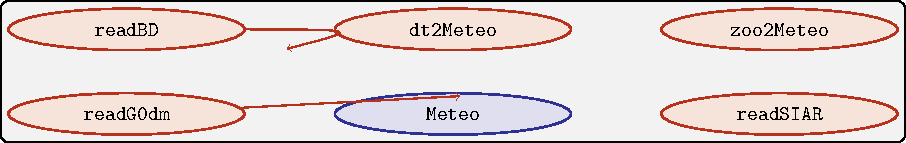
\includegraphics[keepaspectratio,width=\textwidth,height=0.5\textheight]{figuras/calcg0.pdf}
\caption{Cálculo de la radiación incidente en el plano horizontal mediante la función \texttt{calcG0}, la cual procesa un objeto clase \texttt{Sol} y otro clase \texttt{Meteo} mediante las funciones \texttt{fCompD} y \texttt{fCompI} resultando en un objeto clase \texttt{G0}. :\label{fig:calcg0}}
\end{figure}
\begin{itemize}
\item \texttt{fCompD}: La cual computa todas las componentes de la irradiación diaria en una superficie horizontal mediante regresiones entre los parámetros del índice de claridad y la fracción difusa.
Para ello se pueden usar varias correlaciones dependiendo del tipo de datos:
\begin{itemize}
\item Mensuales:
\end{itemize}
\begin{lstlisting}[numbers=left,language=r,label= ,caption= ,captionpos=b]
lat <- 37.2
BTd <- fBTd(mode = 'prom')
solD <- fSolD(lat, BTd)
G0d <- c(2.766,3.491,4.494,5.912,6.989,7.742,7.919,7.027,5.369,3.562,2.814,2.179) * 1000
compD_page <- fCompD(sol = solD, G0d = G0d, corr = "Page")
compD_page
\end{lstlisting}

\begin{verbatim}
Key: <Dates>
	 Dates        Fd        Kt   G0d      D0d      B0d
	<POSc>     <num>     <num> <num>    <num>    <num>
 1: 2024-01-17 0.3404548 0.5836683  2766  941.698 1824.302
 2: 2024-02-14 0.3572461 0.5688088  3491 1247.146 2243.854
 3: 2024-03-15 0.3719989 0.5557532  4494 1671.763 2822.237
 4: 2024-04-15 0.3266485 0.5958862  5912 1931.146 3980.854
 5: 2024-05-15 0.2895069 0.6287549  6989 2023.364 4965.636
 6: 2024-06-10 0.2441221 0.6689185  7742 1889.994 5852.006
 7: 2024-07-18 0.2050844 0.7034651  7919 1624.064 6294.936
 8: 2024-08-18 0.2202349 0.6900576  7027 1547.591 5479.409
 9: 2024-09-18 0.2869638 0.6310055  5369 1540.708 3828.292
10: 2024-10-19 0.3858825 0.5434669  3562 1374.513 2187.487
11: 2024-11-18 0.3578392 0.5682839  2814 1006.959 1807.041
12: 2024-12-13 0.4253038 0.5085807  2179  926.737 1252.263
\end{verbatim}

\begin{lstlisting}[numbers=left,language=r,label= ,caption= ,captionpos=b]
compD_lj <- fCompD(sol = solD, G0d = G0d, corr = "LJ")
compD_lj
\end{lstlisting}

\begin{verbatim}
Key: <Dates>
	 Dates        Fd        Kt   G0d       D0d      B0d
	<POSc>     <num>     <num> <num>     <num>    <num>
 1: 2024-01-17 0.3058193 0.5836683  2766  845.8961 1920.104
 2: 2024-02-14 0.3169470 0.5688088  3491 1106.4621 2384.538
 3: 2024-03-15 0.3268047 0.5557532  4494 1468.6603 3025.340
 4: 2024-04-15 0.2967018 0.5958862  5912 1754.1011 4157.899
 5: 2024-05-15 0.2720419 0.6287549  6989 1901.3006 5087.699
 6: 2024-06-10 0.2408700 0.6689185  7742 1864.8154 5877.185
 7: 2024-07-18 0.2152460 0.7034651  7919 1704.5331 6214.467
 8: 2024-08-18 0.2236251 0.6900576  7027 1571.4138 5455.586
 9: 2024-09-18 0.2703347 0.6310055  5369 1451.4268 3917.573
10: 2024-10-19 0.3361895 0.5434669  3562 1197.5071 2364.493
11: 2024-11-18 0.3173415 0.5682839  2814  892.9990 1921.001
12: 2024-12-13 0.3637158 0.5085807  2179  792.5367 1386.463
\end{verbatim}

\begin{itemize}
\item Diarios:
\end{itemize}
\begin{lstlisting}[numbers=left,language=r,label= ,caption= ,captionpos=b]
G0d <- readSIAR(Lat = 40.40596822621351, Lon =-3.70038308516172,
                inicio = '2024-07-15', final = '2024-08-01',
                tipo = 'Diarios', n_est = 3)
sol <- calcSol(lat, BTd = indexD(G0d))
compD_cpr <- fCompD(sol = sol, G0d = G0d, corr = "CPR")
compD_cpr
\end{lstlisting}

\begin{verbatim}
Key: <Dates>
	 Dates        Fd        Kt      G0d      D0d      B0d
	<POSc>     <num>     <num>    <num>    <num>    <num>
 1: 2024-07-15 0.2833125 0.6798139 7697.945 2180.924 5517.021
 2: 2024-07-16 0.2597185 0.7000272 7911.858 2054.856 5857.002
 3: 2024-07-17 0.2815044 0.6812283 7684.293 2163.163 5521.131
 4: 2024-07-18 0.6627754 0.4674993 5262.702 3487.989 1774.713
 5: 2024-07-19 0.2595844 0.7001561 7865.166 2041.675 5823.491
 6: 2024-07-20 0.2594075 0.7003266 7849.961 2036.339 5813.622
 7: 2024-07-21 0.2315068 0.7365959 8237.938 1907.138 6330.799
 8: 2024-07-22 0.2269337 0.7493438 8361.056 1897.406 6463.650
 9: 2024-07-23 0.2451723 0.7156288 7965.753 1952.982 6012.771
10: 2024-07-24 0.2620008 0.6978638 7748.845 2030.204 5718.641
11: 2024-07-25 0.2746548 0.6867564 7606.140 2089.063 5517.077
12: 2024-07-26 0.3320728 0.6462270 7138.548 2370.518 4768.030
13: 2024-07-27 0.3186769 0.6547900 7213.697 2298.839 4914.858
14: 2024-07-28 0.2767163 0.6850625 7526.355 2082.665 5443.689
15: 2024-07-29 0.6566999 0.4709412 5159.260 3388.086 1771.174
16: 2024-07-30 0.3185533 0.6548709 7153.359 2278.726 4874.633
17: 2024-07-31 0.2503814 0.7096003 7728.034 1934.956 5793.078
18: 2024-08-01 0.2428514 0.7185406 7801.435 1894.589 5906.846
\end{verbatim}

\begin{lstlisting}[numbers=left,language=r,label= ,caption= ,captionpos=b]
compD_ekdd <- fCompD(sol = sol, G0d = G0d, corr = 'EKDd')
compD_ekdd
\end{lstlisting}

\begin{verbatim}
Key: <Dates>
	 Dates    Fd        Kt      G0d      D0d   B0d
	<POSc> <num>     <num>    <num>    <num> <num>
 1: 2024-07-15     1 0.6798139 7697.945 7697.945     0
 2: 2024-07-16     1 0.7000272 7911.858 7911.858     0
 3: 2024-07-17     1 0.6812283 7684.293 7684.293     0
 4: 2024-07-18     1 0.4674993 5262.702 5262.702     0
 5: 2024-07-19     1 0.7001561 7865.166 7865.166     0
 6: 2024-07-20     1 0.7003266 7849.961 7849.961     0
 7: 2024-07-21     1 0.7365959 8237.938 8237.938     0
 8: 2024-07-22     1 0.7493438 8361.056 8361.056     0
 9: 2024-07-23     1 0.7156288 7965.753 7965.753     0
10: 2024-07-24     1 0.6978638 7748.845 7748.845     0
11: 2024-07-25     1 0.6867564 7606.140 7606.140     0
12: 2024-07-26     1 0.6462270 7138.548 7138.548     0
13: 2024-07-27     1 0.6547900 7213.697 7213.697     0
14: 2024-07-28     1 0.6850625 7526.355 7526.355     0
15: 2024-07-29     1 0.4709412 5159.260 5159.260     0
16: 2024-07-30     1 0.6548709 7153.359 7153.359     0
17: 2024-07-31     1 0.7096003 7728.034 7728.034     0
18: 2024-08-01     1 0.7185406 7801.435 7801.435     0
\end{verbatim}

\begin{lstlisting}[numbers=left,language=r,label= ,caption= ,captionpos=b]
compD_climedd <- fCompD(sol = sol, G0d = G0d, corr = 'CLIMEDd')
compD_climedd
\end{lstlisting}

\begin{verbatim}
Key: <Dates>
	 Dates        Fd        Kt      G0d      D0d      B0d
	<POSc>     <num>     <num>    <num>    <num>    <num>
 1: 2024-07-15 0.2724591 0.6798139 7697.945 2097.375 5600.570
 2: 2024-07-16 0.2455880 0.7000272 7911.858 1943.057 5968.801
 3: 2024-07-17 0.2705287 0.6812283 7684.293 2078.822 5605.472
 4: 2024-07-18 0.6086148 0.4674993 5262.702 3202.958 2059.744
 5: 2024-07-19 0.2454217 0.7001561 7865.166 1930.282 5934.884
 6: 2024-07-20 0.2452020 0.7003266 7849.961 1924.826 5925.135
 7: 2024-07-21 0.2013208 0.7365959 8237.938 1658.468 6579.470
 8: 2024-07-22 0.1873678 0.7493438 8361.056 1566.592 6794.463
 9: 2024-07-23 0.2259736 0.7156288 7965.753 1800.050 6165.703
10: 2024-07-24 0.2483878 0.6978638 7748.845 1924.718 5824.126
11: 2024-07-25 0.2630540 0.6867564 7606.140 2000.826 5605.314
12: 2024-07-26 0.3202837 0.6462270 7138.548 2286.361 4852.187
13: 2024-07-27 0.3077503 0.6547900 7213.697 2220.018 4993.679
14: 2024-07-28 0.2653324 0.6850625 7526.355 1996.986 5529.369
15: 2024-07-29 0.6029930 0.4709412 5159.260 3110.998 2048.263
16: 2024-07-30 0.3076331 0.6548709 7153.359 2200.610 4952.749
17: 2024-07-31 0.2334298 0.7096003 7728.034 1803.954 5924.080
18: 2024-08-01 0.2224291 0.7185406 7801.435 1735.266 6066.168
\end{verbatim}

También, se puede aportar una función de corrección propia.
\begin{lstlisting}[numbers=left,language=r,label= ,caption= ,captionpos=b]
f_corrd <- function(sol, G0d){
  ## Función CLIMEDd
    Kt <- Ktd(sol, G0d)
    Fd=(Kt<=0.13)*(0.952)+
    (Kt>0.13 & Kt<=0.8)*(0.868+1.335*Kt-5.782*Kt^2+3.721*Kt^3)+
      (Kt>0.8)*0.141
  return(data.table(Fd, Kt))
}
compD_user <- fCompD(sol = sol, G0d = G0d, corr = 'user', f = f_corrd)
compD_user
\end{lstlisting}

\begin{verbatim}
Key: <Dates>
	 Dates        Fd        Kt      G0d      D0d      B0d
	<POSc>     <num>     <num>    <num>    <num>    <num>
 1: 2024-07-15 0.2724591 0.6798139 7697.945 2097.375 5600.570
 2: 2024-07-16 0.2455880 0.7000272 7911.858 1943.057 5968.801
 3: 2024-07-17 0.2705287 0.6812283 7684.293 2078.822 5605.472
 4: 2024-07-18 0.6086148 0.4674993 5262.702 3202.958 2059.744
 5: 2024-07-19 0.2454217 0.7001561 7865.166 1930.282 5934.884
 6: 2024-07-20 0.2452020 0.7003266 7849.961 1924.826 5925.135
 7: 2024-07-21 0.2013208 0.7365959 8237.938 1658.468 6579.470
 8: 2024-07-22 0.1873678 0.7493438 8361.056 1566.592 6794.463
 9: 2024-07-23 0.2259736 0.7156288 7965.753 1800.050 6165.703
10: 2024-07-24 0.2483878 0.6978638 7748.845 1924.718 5824.126
11: 2024-07-25 0.2630540 0.6867564 7606.140 2000.826 5605.314
12: 2024-07-26 0.3202837 0.6462270 7138.548 2286.361 4852.187
13: 2024-07-27 0.3077503 0.6547900 7213.697 2220.018 4993.679
14: 2024-07-28 0.2653324 0.6850625 7526.355 1996.986 5529.369
15: 2024-07-29 0.6029930 0.4709412 5159.260 3110.998 2048.263
16: 2024-07-30 0.3076331 0.6548709 7153.359 2200.610 4952.749
17: 2024-07-31 0.2334298 0.7096003 7728.034 1803.954 5924.080
18: 2024-08-01 0.2224291 0.7185406 7801.435 1735.266 6066.168
\end{verbatim}

Por último, si \texttt{G0d} ya contiene todos los componentes, se puede especifica que no haga ninguna corrección.
\begin{lstlisting}[numbers=left,language=r,label= ,caption= ,captionpos=b]
compD_none <- fCompD(sol = sol, G0d = compD_user, corr = 'none')
compD_none
\end{lstlisting}

\begin{verbatim}
Key: <Dates>
	 Dates        Fd        Kt      G0d      D0d      B0d
	<POSc>     <num>     <num>    <num>    <num>    <num>
 1: 2024-07-15 0.2724591 0.6798139 7697.945 2097.375 5600.570
 2: 2024-07-16 0.2455880 0.7000272 7911.858 1943.057 5968.801
 3: 2024-07-17 0.2705287 0.6812283 7684.293 2078.822 5605.472
 4: 2024-07-18 0.6086148 0.4674993 5262.702 3202.958 2059.744
 5: 2024-07-19 0.2454217 0.7001561 7865.166 1930.282 5934.884
 6: 2024-07-20 0.2452020 0.7003266 7849.961 1924.826 5925.135
 7: 2024-07-21 0.2013208 0.7365959 8237.938 1658.468 6579.470
 8: 2024-07-22 0.1873678 0.7493438 8361.056 1566.592 6794.463
 9: 2024-07-23 0.2259736 0.7156288 7965.753 1800.050 6165.703
10: 2024-07-24 0.2483878 0.6978638 7748.845 1924.718 5824.126
11: 2024-07-25 0.2630540 0.6867564 7606.140 2000.826 5605.314
12: 2024-07-26 0.3202837 0.6462270 7138.548 2286.361 4852.187
13: 2024-07-27 0.3077503 0.6547900 7213.697 2220.018 4993.679
14: 2024-07-28 0.2653324 0.6850625 7526.355 1996.986 5529.369
15: 2024-07-29 0.6029930 0.4709412 5159.260 3110.998 2048.263
16: 2024-07-30 0.3076331 0.6548709 7153.359 2200.610 4952.749
17: 2024-07-31 0.2334298 0.7096003 7728.034 1803.954 5924.080
18: 2024-08-01 0.2224291 0.7185406 7801.435 1735.266 6066.168
\end{verbatim}

\item \texttt{fCompI}: calcula, en base a los valores de irradiación diaria, todas las componentes de irradiancia. Se vale de dos procedimientos en base al tipo de argumentos que toma:
\begin{itemize}
\item \texttt{compD}: Si recibe un \texttt{data.table} resultado de \texttt{fCompD}, computa las relaciones entre las componentes de irradiancia e irradiación de las componentes de difusa y global, obteniendo con ellas un perfil de irradiancias [\ref{sec:radiacion-superficies-inclinadas}] (las irradiancias global y difusa salen de estas relaciones, mientras que la directa surge por diferencia entre las dos).
\end{itemize}
\begin{lstlisting}[numbers=left,language=r,label= ,caption= ,captionpos=b]
sol <- calcSol(lat = 37.2, BTd = fBTd(mode = 'prom'),
               sample = 'hour', keep.night = FALSE)
G0d <- c(2.766,3.491,4.494,5.912,6.989,7.742,7.919,
          7.027,5.369,3.562,2.814,2.179) * 1000
compD <- fCompD(sol = sol, G0d = G0d, corr = 'CPR')
compI <- fCompI(sol = sol, compD = compD)
show(compI)
\end{lstlisting}

\begin{verbatim}
Key: <Dates>
		   Dates        Fd        Kt        G0        D0        B0
		  <POSc>     <num>     <num>     <num>     <num>     <num>
  1: 2024-01-17 08:00:00 0.5656199 0.4583592  84.06042  47.54625  36.40399
  2: 2024-01-17 09:00:00 0.4912826 0.5277148 215.49558 105.86922 109.51548
  3: 2024-01-17 10:00:00 0.4453619 0.5821268 340.45500 151.62569 188.82159
  4: 2024-01-17 11:00:00 0.4195854 0.6178887 433.04376 181.69885 251.45464
  5: 2024-01-17 12:00:00 0.4098508 0.6325646 473.44106 194.04019 279.57020
 ---                                                                      
141: 2024-12-13 12:00:00 0.5437347 0.5488870 382.71443 208.09513 174.85828
142: 2024-12-13 13:00:00 0.5556284 0.5371376 352.10710 195.64071 156.62669
143: 2024-12-13 14:00:00 0.5893861 0.5063725 276.60890 163.02945 113.57257
144: 2024-12-13 15:00:00 0.6506594 0.4586869 172.87432 112.48231  60.23704
145: 2024-12-13 16:00:00 0.7511394 0.3973283  63.15968  47.44173  15.57107
\end{verbatim}

\begin{itemize}
\item \texttt{G0I}: Este argumento recibe datos de irradiancia, para después, poder aplicar las correcciones indicadas en el argumento \texttt{corr}.
\end{itemize}
\begin{lstlisting}[numbers=left,language=r,label= ,caption= ,captionpos=b]
G0I <- compI$G0
compI_ekdh <- fCompI(sol = sol, G0I = G0I, corr = 'EKDh')
show(compI_ekdh)
\end{lstlisting}

\begin{verbatim}
Key: <Dates>
		   Dates        Fd        Kt        G0        D0        B0
		  <POSc>     <num>     <num>     <num>     <num>     <num>
  1: 2024-01-17 08:00:00 0.7417600 0.4583592  84.06042  62.35265  21.70776
  2: 2024-01-17 09:00:00 0.6000150 0.5277148 215.49558 129.30057  86.19500
  3: 2024-01-17 10:00:00 0.4791716 0.5821268 340.45500 163.13636 177.31865
  4: 2024-01-17 11:00:00 0.4004462 0.6178887 433.04376 173.41074 259.63302
  5: 2024-01-17 12:00:00 0.3692679 0.6325646 473.44106 174.82659 298.61447
 ---                                                                      
141: 2024-12-13 12:00:00 0.5533972 0.5488870 382.71443 211.79307 170.92135
142: 2024-12-13 13:00:00 0.5793829 0.5371376 352.10710 204.00484 148.10226
143: 2024-12-13 14:00:00 0.6457949 0.5063725 276.60890 178.63262  97.97628
144: 2024-12-13 15:00:00 0.7411461 0.4586869 172.87432 128.12512  44.74920
145: 2024-12-13 16:00:00 0.8439123 0.3973283  63.15968  53.30123   9.85845
\end{verbatim}

\begin{lstlisting}[numbers=left,language=r,label= ,caption= ,captionpos=b]
compI_brl <- fCompI(sol = sol, G0I = G0I, corr = 'BRL')
show(compI_brl)
\end{lstlisting}

\begin{verbatim}
Key: <Dates>
		   Dates        Fd        Kt        G0        D0        B0
		  <POSc>     <num>     <num>     <num>     <num>     <num>
  1: 2024-01-17 08:00:00 0.6573908 0.4583592  84.06042  55.26054  28.79987
  2: 2024-01-17 09:00:00 0.5624767 0.5277148 215.49558 121.21125  94.28433
  3: 2024-01-17 10:00:00 0.4845081 0.5821268 340.45500 164.95322 175.50179
  4: 2024-01-17 11:00:00 0.4333714 0.6178887 433.04376 187.66880 245.37496
  5: 2024-01-17 12:00:00 0.4120068 0.6325646 473.44106 195.06094 278.38012
 ---                                                                      
141: 2024-12-13 12:00:00 0.5776181 0.5488870 382.71443 221.06278 161.65164
142: 2024-12-13 13:00:00 0.5917966 0.5371376 352.10710 208.37580 143.73130
143: 2024-12-13 14:00:00 0.6306611 0.5063725 276.60890 174.44649 102.16241
144: 2024-12-13 15:00:00 0.6887448 0.4586869 172.87432 119.06629  53.80803
145: 2024-12-13 16:00:00 0.7561974 0.3973283  63.15968  47.76119  15.39849
\end{verbatim}

\begin{lstlisting}[numbers=left,language=r,label= ,caption= ,captionpos=b]
compI_climedh <- fCompI(sol = sol, G0I = G0I, corr = 'CLIMEDh')
show(compI_climedh)
\end{lstlisting}

\begin{verbatim}
Key: <Dates>
		   Dates        Fd        Kt        G0        D0        B0
		  <POSc>     <num>     <num>     <num>     <num>     <num>
  1: 2024-01-17 08:00:00 0.7093252 0.4583592  84.06042  59.62617  24.43424
  2: 2024-01-17 09:00:00 0.5818534 0.5277148 215.49558 125.38683  90.10875
  3: 2024-01-17 10:00:00 0.4782729 0.5821268 340.45500 162.83039 177.62462
  4: 2024-01-17 11:00:00 0.4110389 0.6178887 433.04376 177.99784 255.04592
  5: 2024-01-17 12:00:00 0.3840268 0.6325646 473.44106 181.81406 291.62701
 ---                                                                      
141: 2024-12-13 12:00:00 0.5416063 0.5488870 382.71443 207.28055 175.43387
142: 2024-12-13 13:00:00 0.5639749 0.5371376 352.10710 198.57956 153.52754
143: 2024-12-13 14:00:00 0.6220088 0.5063725 276.60890 172.05317 104.55573
144: 2024-12-13 15:00:00 0.7087489 0.4586869 172.87432 122.52448  50.34984
145: 2024-12-13 16:00:00 0.8099691 0.3973283  63.15968  51.15739  12.00229
\end{verbatim}

Como con \texttt{fCompD}, se puede añadir una función correctora propia.
\begin{lstlisting}[numbers=left,language=r,label= ,caption= ,captionpos=b]
f_corri <- function(sol, G0i){
  ## Función CLIMEDh
  Kt <- Kti(sol, G0i)
  Fd=(Kt<=0.21)*(0.995-0.081*Kt)+
    (Kt>0.21 & Kt<=0.76)*(0.724+2.738*Kt-8.32*Kt^2+4.967*Kt^3)+
    (Kt>0.76)*0.180
  return(data.table(Fd, Kt))
}
compI_user <- fCompI(sol = sol, G0I = G0I, corr = 'user', f = f_corri)
show(compI_user)
\end{lstlisting}

\begin{verbatim}
Key: <Dates>
		   Dates        Fd        Kt        G0        D0        B0
		  <POSc>     <num>     <num>     <num>     <num>     <num>
  1: 2024-01-17 08:00:00 0.7093252 0.4583592  84.06042  59.62617  24.43424
  2: 2024-01-17 09:00:00 0.5818534 0.5277148 215.49558 125.38683  90.10875
  3: 2024-01-17 10:00:00 0.4782729 0.5821268 340.45500 162.83039 177.62462
  4: 2024-01-17 11:00:00 0.4110389 0.6178887 433.04376 177.99784 255.04592
  5: 2024-01-17 12:00:00 0.3840268 0.6325646 473.44106 181.81406 291.62701
 ---                                                                      
141: 2024-12-13 12:00:00 0.5416063 0.5488870 382.71443 207.28055 175.43387
142: 2024-12-13 13:00:00 0.5639749 0.5371376 352.10710 198.57956 153.52754
143: 2024-12-13 14:00:00 0.6220088 0.5063725 276.60890 172.05317 104.55573
144: 2024-12-13 15:00:00 0.7087489 0.4586869 172.87432 122.52448  50.34984
145: 2024-12-13 16:00:00 0.8099691 0.3973283  63.15968  51.15739  12.00229
\end{verbatim}

Y además, se puede no añadir corrección.
\begin{lstlisting}[numbers=left,language=r,label= ,caption= ,captionpos=b]
G0I <- compI_user
compI_none <- fCompI(sol = sol, G0I = G0I, corr = 'none')
show(compI_none)
\end{lstlisting}

\begin{verbatim}
Key: <Dates>
		   Dates        Fd        Kt        G0        D0        B0
		  <POSc>     <num>     <num>     <num>     <num>     <num>
  1: 2024-01-17 08:00:00 0.7093252 0.4583592  84.06042  59.62617  24.43424
  2: 2024-01-17 09:00:00 0.5818534 0.5277148 215.49558 125.38683  90.10875
  3: 2024-01-17 10:00:00 0.4782729 0.5821268 340.45500 162.83039 177.62462
  4: 2024-01-17 11:00:00 0.4110389 0.6178887 433.04376 177.99784 255.04592
  5: 2024-01-17 12:00:00 0.3840268 0.6325646 473.44106 181.81406 291.62701
 ---                                                                      
141: 2024-12-13 12:00:00 0.5416063 0.5488870 382.71443 207.28055 175.43387
142: 2024-12-13 13:00:00 0.5639749 0.5371376 352.10710 198.57956 153.52754
143: 2024-12-13 14:00:00 0.6220088 0.5063725 276.60890 172.05317 104.55573
144: 2024-12-13 15:00:00 0.7087489 0.4586869 172.87432 122.52448  50.34984
145: 2024-12-13 16:00:00 0.8099691 0.3973283  63.15968  51.15739  12.00229
\end{verbatim}

Por útlimo, esta función incluye un argumento extra, \texttt{filterG0} que cuando su valor es \texttt{TRUE}, elimina todos aquellos valores de irradiancia que son mayores que la irradiancia extra-atmosfércia (ya que es incoherente que la irradiancia terrestre sea mayor que la extra-terrestre)
\end{itemize}

Estas dos funciones, como se muestra en la figura \ref{fig:calcg0}, convergen en la función constructora \texttt{calcG0}, dando como resultado un objeto de clase \texttt{G0}. Este objeto muestra la media mensual de la irradiación diaria y la irradiación anual. A parte incluye los resultados de \texttt{fCompD} y \texttt{fCompI} y los objetos \texttt{Sol} y \texttt{Meteo} de los que parte.

Como argumento más importante está \texttt{modeRad}, el cual selecciona el tipo de datos que introduce el usuario en el argumento \texttt{dataRad}. Estos son:
\begin{itemize}
\item Medias mensuales.
\begin{lstlisting}[numbers=left,language=r,label= ,caption= ,captionpos=b]
G0dm <- c(2.766, 3.491, 4.494, 5.912, 6.989, 7.742, 7.919,
          7.027, 5.369, 3.562, 2.814, 2.179) * 1000
Ta <- c(10, 14.1, 15.6, 17.2, 19.3, 21.2,
       28.4, 29.9, 24.3, 18.2, 17.2, 15.2)
prom <- data.table(G0dm, Ta) 
g0_prom <- calcG0(lat, modeRad = 'prom', dataRad = prom)
show(g0_prom)
\end{lstlisting}

\begin{verbatim}
Object of class  G0 

Source of meteorological information: prom- 

Latitude of source:  37.2 degrees
Latitude for calculations:  37.2 degrees

Monthly avarages:
	Dates   G0d      D0d      B0d
       <char> <num>    <num>    <num>
 1: Jan. 2024 2.766 0.941698 1.824302
 2: Feb. 2024 3.491 1.247146 2.243854
 3: Mar. 2024 4.494 1.671763 2.822237
 4: Apr. 2024 5.912 1.931146 3.980854
 5: May. 2024 6.989 2.023364 4.965636
 6: Jun. 2024 7.742 1.889994 5.852006
 7: Jul. 2024 7.919 1.624064 6.294936
 8: Aug. 2024 7.027 1.547591 5.479409
 9: Sep. 2024 5.369 1.540708 3.828292
10: Oct. 2024 3.562 1.374513 2.187487
11: Nov. 2024 2.814 1.006959 1.807041
12: Dec. 2024 2.179 0.926737 1.252263

Yearly values:
   Dates      G0d      D0d      B0d
   <int>    <num>    <num>    <num>
1:  2024 1839.365 540.6331 1298.732
\end{verbatim}

\item Generación de secuencias diarias mediante matrices de transición de Markov.
\begin{lstlisting}[numbers=left,language=r,label= ,caption= ,captionpos=b]
g0_aguiar <- calcG0(lat, modeRad = 'aguiar', dataRad = prom)
show(g0_aguiar)
\end{lstlisting}

\begin{verbatim}
Object of class  G0 

Source of meteorological information: bd-aguiar 

Latitude of source:  37.2 degrees
Latitude for calculations:  37.2 degrees

Monthly avarages:
	Dates   G0d      D0d      B0d
       <char> <num>    <num>    <num>
 1: Jan. 2024 2.766 1.101143 1.664857
 2: Feb. 2024 3.491 1.519465 1.971535
 3: Mar. 2024 4.494 1.896690 2.597310
 4: Apr. 2024 5.912 2.353760 3.558240
 5: May. 2024 6.989 2.445564 4.543436
 6: Jun. 2024 7.742 2.442996 5.299004
 7: Jul. 2024 7.919 2.238474 5.680526
 8: Aug. 2024 7.027 2.066795 4.960205
 9: Sep. 2024 5.369 2.016564 3.352436
10: Oct. 2024 3.562 1.659453 1.902547
11: Nov. 2024 2.814 1.223016 1.590984
12: Dec. 2024 2.179 1.086253 1.092747

Yearly values:
Key: <Dates>
   Dates      G0d      D0d      B0d
   <int>    <num>    <num>    <num>
1:  2024 1839.365 672.4801 1166.885
\end{verbatim}

\item Diarios.
\begin{lstlisting}[numbers=left,language=r,label= ,caption= ,captionpos=b]
bd <- g0_aguiar@G0D
g0_bd <- calcG0(lat, modeRad = 'bd', dataRad = bd)
show(g0_bd)
\end{lstlisting}

\begin{verbatim}
Object of class  G0 

Source of meteorological information: bd-data.table 

Latitude of source:  37.2 degrees
Latitude for calculations:  37.2 degrees

Monthly avarages:
	Dates   G0d      D0d      B0d
       <char> <num>    <num>    <num>
 1: Jan. 2024 2.766 1.101143 1.664857
 2: Feb. 2024 3.491 1.519465 1.971535
 3: Mar. 2024 4.494 1.896690 2.597310
 4: Apr. 2024 5.912 2.353760 3.558240
 5: May. 2024 6.989 2.445564 4.543436
 6: Jun. 2024 7.742 2.442996 5.299004
 7: Jul. 2024 7.919 2.238474 5.680526
 8: Aug. 2024 7.027 2.066795 4.960205
 9: Sep. 2024 5.369 2.016564 3.352436
10: Oct. 2024 3.562 1.659453 1.902547
11: Nov. 2024 2.814 1.223016 1.590984
12: Dec. 2024 2.179 1.086253 1.092747

Yearly values:
Key: <Dates>
   Dates      G0d      D0d      B0d
   <int>    <num>    <num>    <num>
1:  2024 1839.365 672.4801 1166.885
\end{verbatim}

\item Intradiarios
\begin{lstlisting}[numbers=left,language=r,label= ,caption= ,captionpos=b]
bdI <- g0_aguiar@G0I
g0_bdI <- calcG0(lat, modeRad = 'bdI', dataRad = bdI)
show(g0_bdI)
\end{lstlisting}

\begin{verbatim}
Object of class  G0 

Source of meteorological information: bdI-data.table 

Latitude of source:  37.2 degrees
Latitude for calculations:  37.2 degrees

Monthly avarages:
	Dates   G0d      D0d      B0d
       <char> <num>    <num>    <num>
 1: Jan. 2024 2.766 1.118008 1.647992
 2: Feb. 2024 3.491 1.560352 1.930648
 3: Mar. 2024 4.494 2.016896 2.477104
 4: Apr. 2024 5.912 2.445615 3.466385
 5: May. 2024 6.989 2.500928 4.488072
 6: Jun. 2024 7.742 2.374257 5.367743
 7: Jul. 2024 7.919 1.923060 5.995940
 8: Aug. 2024 7.027 1.826466 5.200534
 9: Sep. 2024 5.369 1.853025 3.515975
10: Oct. 2024 3.562 1.670767 1.891233
11: Nov. 2024 2.814 1.265921 1.548079
12: Dec. 2024 2.179 1.122945 1.056055

Yearly values:
Key: <Dates>
   Dates      G0d      D0d      B0d
   <int>    <num>    <num>    <num>
1:  2024 1839.365 660.9659 1178.399
\end{verbatim}
\end{itemize}

\section{Radiación efectiva en el plano del generador}
\label{sec:org4839347}
\label{sec:radiacion-efectiva-plano-generador}
Teniendo la radiación incidente en plano horizontal (sección \ref{sec:radiacion-plano-horizontal}), se puede calcular la radiación efectiva incidente en el plano del generador. Para ello, \texttt{solaR2} cuenta con la función \texttt{calcGef} [\ref{subsec:calcgef}] la cual mediante las funciones \texttt{fInclin} y \texttt{calcShd} procesa un objeto de clase \texttt{G0} para obtener un objeto \texttt{Gef}.

Como se puede ver en la figura \ref{fig:calcgef}, \texttt{calcG0} funciona gracias a las siguientes funciones:
\begin{figure}[]
\centering
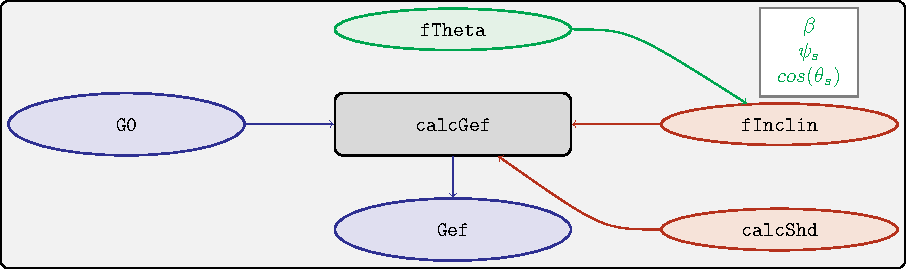
\includegraphics[keepaspectratio,width=\textwidth,height=0.5\textheight]{figuras/calcgef.pdf}
\caption{Cálculo de la radiación efectiva incidente en el plano del generador mediante la función \texttt{calcGef}, la cual emplea la función \texttt{fInclin} para el computo de las componentes efectivas, la función \texttt{fTheta} que provee a la función anterior los ángulos necesarios para su computo y la función \texttt{calcShd} que reprocesa el objeto de clase \texttt{Gef} resultante, añadiendole el efecto de las sombras producidas entres módulos. \label{fig:calcgef}}
\end{figure}
\begin{itemize}
\item \texttt{fTheta}: la cual, partiendo del ángulo de inclinación (\(\beta\)) y la orientación (\(\alpha\)), computa el ángulo de inclinación en cada instante (\(\beta\)), el ángulo azimutal (\(\psi_s\)) y el coseno del ángulo de incidencia  de la radiación solar en la superficie (\(cos(\theta_s)\)).
Como principal argumento tiene \texttt{modeTrk}, el cual determina el sistema de seguimiento que tiene el sistema:
\begin{itemize}
\item \texttt{fixed}: para sistemas estáticos.
\end{itemize}
\begin{lstlisting}[numbers=left,language=r,label= ,caption= ,captionpos=b]
BTd <- fBTd(mode = 'prom')[6] 
sol <- calcSol(lat, BTd = BTd, keep.night = FALSE)
beta <- lat - 10
alfa <- 0
angGen_fixed <- fTheta(sol = sol, beta = beta, alfa = alfa,
                 modeTrk = 'fixed')
show(angGen_fixed)
\end{lstlisting}

\begin{verbatim}
		  Dates      Beta  Alfa   cosTheta
		 <POSc>     <num> <num>      <num>
 1: 2024-06-10 05:00:00 0.4747296     0 0.00000000
 2: 2024-06-10 06:00:00 0.4747296     0 0.06990810
 3: 2024-06-10 07:00:00 0.4747296     0 0.30432148
 4: 2024-06-10 08:00:00 0.4747296     0 0.52263672
 5: 2024-06-10 09:00:00 0.4747296     0 0.70998013
 6: 2024-06-10 10:00:00 0.4747296     0 0.85358815
 7: 2024-06-10 11:00:00 0.4747296     0 0.94367686
 8: 2024-06-10 12:00:00 0.4747296     0 0.97410861
 9: 2024-06-10 13:00:00 0.4747296     0 0.94281011
10: 2024-06-10 14:00:00 0.4747296     0 0.85191372
11: 2024-06-10 15:00:00 0.4747296     0 0.70761218
12: 2024-06-10 16:00:00 0.4747296     0 0.51973665
13: 2024-06-10 17:00:00 0.4747296     0 0.30108697
14: 2024-06-10 18:00:00 0.4747296     0 0.06655958
15: 2024-06-10 19:00:00 0.4747296     0 0.00000000
\end{verbatim}

\begin{itemize}
\item \texttt{two}: para sistemas de seguimiento de doble eje.
\end{itemize}
\begin{lstlisting}[numbers=left,language=r,label= ,caption= ,captionpos=b]
angGen_two <- fTheta(sol = sol, beta = beta, alfa = alfa,
                     modeTrk = 'two')
show(angGen_two)
\end{lstlisting}

\begin{verbatim}
		  Dates      Beta         Alfa cosTheta
		 <POSc>     <num>        <num>    <num>
 1: 2024-06-10 05:00:00 1.5220852 -2.043678875        1
 2: 2024-06-10 06:00:00 1.3300857 -1.896688029        1
 3: 2024-06-10 07:00:00 1.1285281 -1.756655282        1
 4: 2024-06-10 08:00:00 0.9215732 -1.612213267        1
 5: 2024-06-10 09:00:00 0.7134716 -1.445120762        1
 6: 2024-06-10 10:00:00 0.5110180 -1.215351693        1
 7: 2024-06-10 11:00:00 0.3328578 -0.809087856        1
 8: 2024-06-10 12:00:00 0.2466893  0.006963841        1
 9: 2024-06-10 13:00:00 0.3349967  0.817155564        1
10: 2024-06-10 14:00:00 0.5137803  1.219398208        1
11: 2024-06-10 15:00:00 0.7163931  1.447776194        1
12: 2024-06-10 16:00:00 0.9245147  1.614353339        1
13: 2024-06-10 17:00:00 1.1314208  1.758631827        1
14: 2024-06-10 18:00:00 1.3328735  1.898691776        1
15: 2024-06-10 19:00:00 1.5247042  2.045849315        1
\end{verbatim}

\begin{itemize}
\item \texttt{horiz}: para sistemas de seguimiento horizontal Norte-Sur.
\end{itemize}
\begin{lstlisting}[numbers=left,language=r,label= ,caption= ,captionpos=b]
angGen_horiz <- fTheta(sol = sol, beta = beta, alfa = alfa,
                       modeTrk = 'horiz')
show(angGen_horiz)
\end{lstlisting}

\begin{verbatim}
		  Dates        Beta      Alfa  cosTheta
		 <POSc>       <num>     <num>     <num>
 1: 2024-06-10 05:00:00 1.516091993 -1.570796 0.8905353
 2: 2024-06-10 06:00:00 1.317263961 -1.570796 0.9504350
 3: 2024-06-10 07:00:00 1.121771495 -1.570796 0.9859551
 4: 2024-06-10 08:00:00 0.921160041 -1.570796 0.9994560
 5: 2024-06-10 09:00:00 0.709555740 -1.570796 0.9966296
 6: 2024-06-10 10:00:00 0.483954771 -1.570796 0.9854098
 7: 2024-06-10 11:00:00 0.245151627 -1.570796 0.9742418
 8: 2024-06-10 12:00:00 0.001753607  1.570796 0.9697277
 9: 2024-06-10 13:00:00 0.248597042  1.570796 0.9743648
10: 2024-06-10 14:00:00 0.487239436  1.570796 0.9855868
11: 2024-06-10 15:00:00 0.712638107  1.570796 0.9967482
12: 2024-06-10 16:00:00 0.924058412  1.570796 0.9993956
13: 2024-06-10 17:00:00 1.124550569  1.570796 0.9856166
14: 2024-06-10 18:00:00 1.320024608  1.570796 0.9497600
15: 2024-06-10 19:00:00 1.518974473  1.570796 0.8895182
\end{verbatim}

También, tiene un argumento \texttt{BT} que indica cuando se usa la técnica de backtracking para un sistema horizontal Norte-Sur. Para funcionar, necesita de los argumentos \texttt{struct}, el cual presenta una lista con la altura de los módulos, y \texttt{dist}, el cual presenta un \texttt{data.frame} (o \texttt{data.table}) con la distancia que separa los módulos en la dirección Este-Oeste.
\begin{lstlisting}[numbers=left,language=r,label= ,caption= ,captionpos=b]
struct <- list(L = 1)
dist <- data.table(Lew = 2)
angGen_BT <- fTheta(sol = sol, beta = beta, alfa = alfa,
                    modeTrk = 'horiz', BT = TRUE,
                    struct = struct, dist = dist)
show(angGen_BT)
\end{lstlisting}

\begin{verbatim}
		  Dates        Beta      Alfa   cosTheta
		 <POSc>       <num>     <num>      <num>
 1: 2024-06-10 05:00:00 0.054868903 -1.570796 0.09738369
 2: 2024-06-10 06:00:00 0.271972628 -1.570796 0.47678565
 3: 2024-06-10 07:00:00 0.602487004 -1.570796 0.85598103
 4: 2024-06-10 08:00:00 0.921160041 -1.570796 0.99945597
 5: 2024-06-10 09:00:00 0.709555740 -1.570796 0.99662956
 6: 2024-06-10 10:00:00 0.483954771 -1.570796 0.98540983
 7: 2024-06-10 11:00:00 0.245151627 -1.570796 0.97424175
 8: 2024-06-10 12:00:00 0.001753607  1.570796 0.96972767
 9: 2024-06-10 13:00:00 0.248597042  1.570796 0.97436477
10: 2024-06-10 14:00:00 0.487239436  1.570796 0.98558683
11: 2024-06-10 15:00:00 0.712638107  1.570796 0.99674816
12: 2024-06-10 16:00:00 0.924058412  1.570796 0.99939563
13: 2024-06-10 17:00:00 0.595256963  1.570796 0.85074877
14: 2024-06-10 18:00:00 0.268563625  1.570796 0.47136897
15: 2024-06-10 19:00:00 0.051961679  1.570796 0.09215170
\end{verbatim}

\item \texttt{fInclin}: la cual, partiendo del resultado de \texttt{fTheta} y de un objeto de clase \texttt{G0}, cálcula la irradiancia solar incidente en una superficie inclinada junto con los efectos del ángulo de incidencia y la suciedad para obtener la irradiancia efectiva.
Como argumentos principales están:
\begin{itemize}
\item \texttt{iS}: permite seleccionar entre 4 valores del 1 al 4 correspondientes a la suciedad del módulo. Siendo 1 limpio y 4 alto y basandose en los valores de la tabla \ref{tab:coef-perd} computa la irradiancia efectiva.
\end{itemize}
\begin{lstlisting}[numbers=left,language=r,label= ,caption= ,captionpos=b]
compI <- calcG0(lat, dataRad = prom, keep.night = FALSE)
sol <- calcSol(lat, BTi = indexI(compI))
angGen <- fTheta(sol = sol, beta = beta, alfa = alfa)
inclin_limpio <- fInclin(compI = compI, angGen = angGen, iS = 1)
show(inclin_limpio)
\end{lstlisting}

\begin{verbatim}
		   Dates        Bo       Bn        G         D       Di        Dc         B         R
		  <POSc>     <num>    <num>    <num>     <num>    <num>     <num>     <num>     <num>
  1: 2024-01-17 08:00:00  514.5612 365.8727 186.4590  52.34286 25.82073  26.52212 133.18653 0.9295706
  2: 2024-01-17 09:00:00  792.6980 464.2106 366.6704 103.96230 52.12242  51.83988 260.32510 2.3830282
  3: 2024-01-17 10:00:00 1010.9063 541.3602 536.6247 145.69981 68.60264  77.09717 387.15997 3.7648749
  4: 2024-01-17 11:00:00 1154.3223 592.0663 662.0048 173.72247 77.44190  96.28057 483.49354 4.7887550
  5: 2024-01-17 12:00:00 1213.1770 612.8750 716.5974 185.35767 80.61172 104.74595 526.00427 5.2354830
 ---                                                                                                 
141: 2024-12-13 12:00:00 1181.1554 470.2512 578.4583 180.82966 95.85462  84.97504 393.39650 4.2321949
142: 2024-12-13 13:00:00 1129.5610 453.5904 536.8668 170.08970 91.70559  78.38411 362.88341 3.8937280
143: 2024-12-13 14:00:00  994.4636 409.9651 434.0673 142.25355 79.88147  62.37208 288.75488 3.0588416
144: 2024-12-13 15:00:00  785.0640 342.3463 292.1950  99.92831 58.81096  41.11735 190.35496 1.9117069
145: 2024-12-13 16:00:00  515.6229 255.3390 140.8937  46.94651 26.80445  20.14206  93.24874 0.6984426
	     FTb        FTd       FTr     Dief      Dcef      Gef       Def       Bef       Ref
	   <num>      <num>     <num>    <num>     <num>    <num>     <num>     <num>     <num>
  1: 0.115032290 0.05043622 0.2503398 24.51843  23.47122 166.5523  47.98966 117.86578 0.6968621
  2: 0.034235799 0.05043622 0.2503398 49.49356  50.06510 352.7578  99.55866 251.41266 1.7864615
  3: 0.012139104 0.05043622 0.2503398 65.14258  76.16128 526.5864 141.30386 382.46020 2.8223770
  4: 0.005426675 0.05043622 0.2503398 73.53602  95.75809 653.7538 169.29411 480.86978 3.5899392
  5: 0.003640433 0.05043622 0.2503398 76.54597 104.36463 708.9248 180.91060 524.08939 3.9248333
 ---                                                                                           
141: 0.004516349 0.05043622 0.2503398 91.02007  84.59127 570.4038 175.61134 391.61978 3.1727082
142: 0.006269898 0.05043622 0.2503398 87.08031  77.89265 528.5001 164.97296 360.60816 2.9189730
143: 0.013120704 0.05043622 0.2503398 75.85255  61.55372 424.6656 137.40626 284.96622 2.2930919
144: 0.035287438 0.05043622 0.2503398 55.84476  39.66642 280.5821  95.51118 183.63782 1.4331306
145: 0.114223038 0.05043622 0.2503398 25.45254  17.84137 126.4151  43.29391  82.59758 0.5235947
\end{verbatim}
\end{itemize}
